\chapter{Priority Queues \label{chap:prioqueue}}
In order to introduce \href{https://en.wikipedia.org/wiki/Priority_queue}{\emph{priority queues}},
we first take a look at ordinary
\href{https://en.wikipedia.org/wiki/Queue_(abstract_data_type)}{\emph{queues}}.
Basically, a queue can be viewed as a list with the following restrictions:
\begin{enumerate}
\item A new elements can only be appended at the end of the list.
\item Only the element at the beginning of the list can be removed.
\end{enumerate}
This is similar to the queue at a cinema box office.  There, a queue is a long line of people
waiting to buy a ticket.  The person at the front of the queue is served and thereby removed from
the queue.  New persons entering the cinema have to line up at the end of the queue.  In contrast, a
priority queue is more like a dentist's waiting room.  If you have an appointment at 10:00 and you
have already waited for an hour, suddenly a patient with no appointment but a private insurance
shows up.  Since this has a higher priority, this patient will then be attended next while you have
to wait for another hour. 

Priority queues have many applications in computer science.  We will make use of priority queues,
first, when implementing Huffman's algorithm for data compression and, second, when we implement
Dijkstra's algorithm for finding the shortest path in a weighted graph.  Furthermore, priority
queues are used in simulation systems and in operating systems when scheduling processes.


\section[Formal Definition]{Formal Definition of the ADT \textsl{PrioQueue}}
Next, we give a formal definition of the ADT \textsl{PrioQueue}.  Since the data type
\textsl{PrioQueue} is really just an auxiliary data type, the definition we give is somewhat
restricted: We will only specify those functions that are needed for Dijkstra's algorithm.
These functions will also be sufficient for Huffman's algorithm.

\begin{Definition}[Priority Queue] \hspace*{\fill} \\
  The abstract data type of priority queues is defined as follows:
  \begin{enumerate}
  \item The name is \textsl{PrioQueue}.
  \item The set of type parameters is \\[0.1cm]
        \hspace*{1.3cm} $\{ \textsl{Priority}, \textsl{Value} \}$.

        Furtheremore, there must exist a linear ordering $<$ on the set $\textsl{Priority}$.
        This is needed since we want to compare the priority of different elements.
  \item The set of function symbols is \\[0.1cm]
       \hspace*{1.3cm} 
       $\{ \textsl{prioQueue}, \textsl{insert}, \textsl{remove}, \textsl{top} \}$.
  \item The type specifications of these function symbols is given as follows:
        \begin{enumerate}
        \item $\textsl{prioQueue}: \textsl{PrioQueue}$

              The function invocation  ``$\textsl{prioQueue}()$'' creates a new, empty priority queue.
        \item $\textsl{top}: \textsl{PrioQueue}  \rightarrow (\textsl{Priority} \times \textsl{Value}) \cup \{\Omega\}$

              The expression $Q.\textsl{top}()$ returns a pair $\pair(p,v)$.  Here,  $v$ is any
              element of $Q$ that is of maximal priority in $Q$, while $p$ is its priority.
        \item $\textsl{insert}: \textsl{PrioQueue} \times \textsl{Priority} \times \textsl{Value} \rightarrow \textsl{PrioQueue}$

              The expression $Q.\textsl{insert}(p,v)$ inserts the  element $v$ into the priority queue $Q$.
              Furthermore, the priority of $v$ is set to be $p$.
        \item $\textsl{remove}: \textsl{PrioQueue} \rightarrow \textsl{PrioQueue}$

              The expression $Q.\textsl{remove}()$ removes from $Q$ the element that is returned by
              $Q.\texttt{top}()$.
        \end{enumerate}
\item Before we are able to specify the behavior of the functions implementing the function symbols
      given above, we have to discuss the notion of \emph{priority}.  We assume that there exists
      a set $\textsl{Priority}$ and there is a linear order $<$ defined on this set.
      If  $p_1 < p_2$, then the priority $p_1$ is \emph{higher} than the priority $p_2$.  This
      nomenclature might seem counter intuitive.  It is motivated by 
      Dijkstra's algorithm which is discussed later.  In Dijkstra's algorithm, the priorities are
      distances in a graph and the priority of a node is higher if the node is nearer to the source
      node.

      Next, the behavior of the functions is specified via a reference implementation.  We demand
      that the behavior of the functions making up the ADT \textsl{PrioQueue} is the same
      as the behavior of the reference implementation.
      
      In our reference implementation a priority queue is implemented as a set of pairs of the form 
      $\pair(p,v)$ where $p$ is a priority, while $v$ is a value.  The reference implementation
      proceeds as follows:
      \begin{enumerate}
      \item $\textsl{prioQueue}() = \{\}$

            The constructor returns an empty priority queue.
      \item $Q.\textsl{insert}(p, v) = Q \cup \{ \pair(p,v) \}$,
        
            In order to insert an  element $v$ with priority $p$ into the priority queue 
            $Q$ it is sufficient to add the pair $\pair(p,v)$ to the set $Q$.
      \item If  $Q$ is empty, then $Q.\textsl{top}()$ is undefined: \\[0.1cm]
            \hspace*{1.3cm} $Q = \{\} \;\rightarrow\; Q.\textsl{top}() = \Omega$.
     \item If $Q$ is not empty, then the expression $Q.\textsl{top}()$ returns a pair $\pair(p_2,v)$
           from the set such that $p_2$ has the highest priority.  Hence we must have:
              \\[0.1cm]
              \hspace*{1.3cm} 
              $\pair(p_1,v_1) \in Q \;\wedge\; Q.\textsl{top}() = \pair(p_2,v_2)
              \;\rightarrow\; p_2 \leq p_1 \;\wedge\; \pair(p_2,v_2) \in Q$.
      \item If  $Q$ is empty, then calling $\textsl{remove}()$ does not change this fact: \\[0.1cm]
            \hspace*{1.3cm} $Q = \{\} \rightarrow Q.\textsl{remove}() = Q$.
      \item Otherwise,  $Q.\textsl{remove}()$ removes the pair form $Q$ that is returned by $Q.\textsl{top}()$: \\[0.1cm]
            \hspace*{1.3cm} 
            $Q \not= \{\} \rightarrow Q.\textsl{remove}() = Q \backslash \bigl\{ Q.\textsl{top}() \bigr\}$.
      \end{enumerate}
\end{enumerate}
\end{Definition}
We could implement the ADT \textsl{PrioQueue} as a list of pairs that is sorted ascendingly.
Then, the different methods of \textsl{PrioQueue} would be implemented as follows:
\begin{enumerate}
\item $\textsl{prioQueue}()$ returns an empty list.
\item $Q.\textsl{insert}(d)$ can be implemented via the function  \texttt{insert} that we have
      used when implementing the algorithm ``\emph{insertion sort}''.
\item $Q.\textsl{top}()$ return the first element from the list $Q$.
\item $Q.\textsl{remove}()$ removes the first element from $Q$.
\end{enumerate}
The worst case complexity of this approach would be linear for the method $\textsl{insert}()$,
i.e.~it would have complexity $\Oh(n)$ where $n$ is the number of elements in $Q$. 
All other operations would have the complexity $\Oh(1)$.  
Next, we introduce a more efficient implementation such that the complexity of $\textsl{insert}()$ 
is only $\Oh\bigl(\log(n)\bigr)$.  To this end, we introduce
\href{https://en.wikipedia.org/wiki/Heap_(data_structure)}{\emph{Heaps}} next. 

\section[Heaps]{The \emph{Heap} Data Structure}
We define the set \href{https://en.wikipedia.org/wiki/Heap_(data_structure)}{\textsl{Heap}}\footnote{
In computer science, the notion of a \textsl{Heap} is used for two different concepts:
First, a \emph{heap} is a data structure that is organized as a tree.  This kind of data structure
is described in more detail in this section. Second, the part of main memory that contains dynamically
allocated objects is known as \emph{the heap}.}
inductively as a subset of the set $\Bin$ of binary trees.  To this end, we first define a relation
\\[0.2cm]
\hspace*{1.3cm}
$\leq \;\subseteq \textsl{Priority}  \times \mathcal{B}$
\\[0.2cm]
For a priority $p \in \textsl{Priority}$ and a binary tree $b \in \Bin$ we have  $p \leq b$ 
if and only if $p \leq q$ for every priority $q$ occurring in $b$.  The formal definition of 
$p \leq b$ is as follows:
\begin{enumerate}
\item $p \leq \textsl{Nil}$,

      because there are no priorities in the empty tree \textsl{Nil}.
\item $p \leq \textsl{Node}(q,v,l,r) \;\stackrel{\mbox{\scriptsize def}}{\longleftrightarrow}\; p \leq q \;\wedge\; p \leq l \;\wedge\; p \leq r$,
         
      because $p$ is less than or equal to every priority in the binary tree 
      $\textsl{Node}(q,v,l,r)$ iff  $p \leq q$ and if, furthermore, 
      $p$ is less than or equal to every priority occurring in either  $l$ or $r$.
\end{enumerate}
Next, we define a function \\[0.1cm]
\hspace*{1.3cm} $\textsl{count}: \Bin \rightarrow \mathbb{N}_0$, \\[0.1cm]
that counts the number of nodes occurring in a binary tree $b$.  The definition of
$b.\textsl{count}()$ is given by induction on $b$.
\begin{enumerate}
\item $\textsl{Nil}.\textsl{count}() = 0$.
\item $\textsl{Node}(p,v,l,r).\textsl{count}() = 1 + l.\textsl{count}() + r.\textsl{count}()$.
\end{enumerate}
Now we are ready to define the set \textsl{Heap} by induction:
\begin{enumerate}
\item $\textsl{Nil} \in \textsl{Heap}$.
\item $\textsl{Node}(p,v,l,r) \in \textsl{Heap}$ if and only if the following is true:
      \begin{enumerate}
      \item $p \leq l \;\wedge\; p \leq r$

            The priority stored at the root is less than or equal to every other priority stored in
            the heap. This condition is known as the \emph{heap condition}.
      \item $\mid l.\textsl{count}() - r.\textsl{count}() \mid \;\leq\, 1$

            The number of elements in the left subtree differs from the number of elements stored in
            the right subtree by at most one.
            This condition is known as the  \emph{balancing condition}.  It is similar to the
            balancing condition of AVL trees, but instead of comparing the heights, this condition
            compares the number of elements.
      \item $l \in \textsl{Heap} \;\wedge\; r \in \textsl{Heap}$

            This condition ensures that all subtrees are heaps, too.
      \end{enumerate}
\end{enumerate}
The  \emph{heap condition} implies that in a non-empty heap the element with a highest priority is
stored at the root.  Figure \ref{fig:heap-list} on page \pageref{fig:heap-list} shows a simple heap.
In the upper part of the nodes we find the priorities.  Below these priorities we have the values
that are stored in the heap.  In the example given, the priorities are natural numbers, while the
values are characters.


\begin{figure}[!t]
  \centering
  \framebox{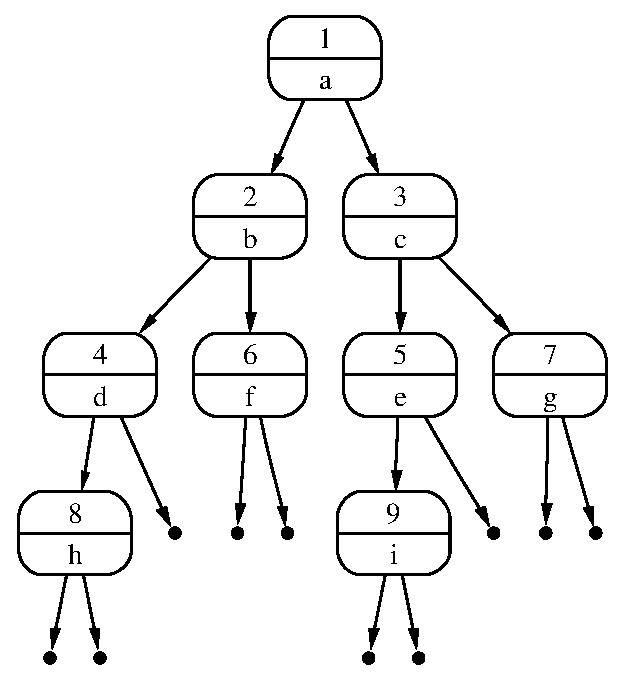
\epsfig{file=Abbildungen/heap-with-holes,scale=0.7}} 
  \caption{Ein Heap}
  \label{fig:heap-list}
\end{figure}

As heaps are binary trees, we can implements them in a fashion that is similar to our implementation
of AVL trees.  In order to do so, we first present equations that specify the methods of the data
structure heap.  We start with the method \textsl{top}.  
\begin{enumerate}
\item $\textsl{Nil}.\textsl{top}() = \Omega$.
\item $\textsl{Node}(p,v,l,r).\textsl{top}() = \pair(p,v)$,

      because the heap condition ensures that the value with the highest priority is stored at the
      top. 
\end{enumerate}
When  implementing the method \textsl{insert} we have to make sure that both the balancing condition
and the heap condition are maintained.
\begin{enumerate}
\item $\textsl{Nil}.\textsl{insert}(p,v) = \textsl{Node}(p,v,\textsl{Nil}, \textsl{Nil})$.
\item $p_{\mathrm{top}} \leq p \;\wedge\; l.\textsl{count}() \leq r.\textsl{count}() \;\rightarrow $   \\[0.1cm]
      \hspace*{1.3cm} 
      $\textsl{Node}(p_{\mathrm{top}},v_\mathrm{top},l,r).\textsl{insert}(p,v) =
                 \textsl{Node}\bigl(p_\mathrm{top},v_\mathrm{top},l.\textsl{insert}(p,v), r\bigr)$.
                 
      If the value $v$ to be inserted has a priority that is lower (or the same) than the priority of
      the value at the root of the heap, we have to insert the value $v$ either in the left or right
      subtree.  In order to maintain the balancing condition, we insert the value $v$ in the left
      subtree if that subtree stores at most as many values as the right subtree.
\item $p_{\mathrm{top}} \leq p \;\wedge\; l.\textsl{count}() > r.\textsl{count}() \;\rightarrow $   \\[0.1cm]
      \hspace*{1.3cm} 
      $\textsl{Node}(p_{\mathrm{top}},v_\mathrm{top},l,r).\textsl{insert}(p,v) =
                 \textsl{Node}\bigl(p_\mathrm{top},v_\mathrm{top},l,r.\textsl{insert}(p,v)\bigr)$.

      If the value $v$ to be inserted has a priority that is lower (or the same) than the priority of
      the value at the root of the heap, we have to insert the value $v$ in the right
      subtree if the right subtree  stores fewer values than the left subtree.
\item $p_{\mathrm{top}} > p \;\wedge\; l.\textsl{count}() \leq r.\textsl{count}() \;\rightarrow $ \\[0.1cm]
      \hspace*{1.3cm} 
      $\textsl{Node}(p_{\mathrm{top}},v_\mathrm{top},l,r).\textsl{insert}(p,v) =
                 \textsl{Node}\bigl(p,v,l.\textsl{insert}(p_\mathrm{top},v_\mathrm{top}), r\bigr)$.

      If the value $v$ to be inserted is associated with a priority $p$ that is higher than the priority of
      the value stored at the root of the heap, then we have to store the value $v$ at the root.
      The value $v_\mathrm{top}$ that was stored previously at the root has to be moved to either
      the left or right subtree.  If the number of nodes in the left subtree is as most as big as
      the number of nodes in the right subtree, $v_\mathrm{top}$ is inserted into the left subtree.
\item $p_{\mathrm{top}} > p \;\wedge\; l.\textsl{count}() > r.\textsl{count}() \;\rightarrow $ \\[0.1cm] 
      \hspace*{1.3cm} 
      $\textsl{Node}(p_{\mathrm{top}},v_\mathrm{top},l,r).\textsl{insert}(p,v) =
                 \textsl{Node}\bigl(p,v,l,r.\textsl{insert}(p_\mathrm{top},v_\mathrm{top})\bigr)$.

      If the value $v$ to be inserted is associated with a priority $p$ that is higher than the priority of
      the value stored at the root of the heap, then we have to store the value $v$ at the root.
      The value $v_\mathrm{top}$ that was stored previously at the root has to be moved to 
      the right subtree provided the number of nodes in the left subtree bigger than
      the number of nodes in the right subtree.
\end{enumerate}
Finally, we specify our implementation of the method \textsl{remove}.
\begin{enumerate}
\item $\textsl{Nil}.\textsl{remove}() = \textsl{Nil}$,

      since we cannot remove anything from the empty heap.
\item $\textsl{Node}(p,v,\textsl{Nil},r).\textsl{remove}() = r$,
  
\item $\textsl{Node}(p,v,l,\textsl{Nil}).\textsl{remove}() = l$,

      because we always remove the value with the highest priority and this value is stored at the
      root.  Now if either of the two subtrees is empty, we can just return the other subtree.

      Next, we discuss those cases where none of the subtrees is empty.
      In that case, either the value that is stored at the root of the left subtree or the value
      stored at the root of the right subtree has to be promoted to the root of the tree.
      In order to maintain the heap condition, we have to take the value that is associated with the
      higher priority.
\item $p_1 \leq p_2 \;\wedge\; l = \textsl{Node}(p_1,v_1,l_1,r_1) \;\wedge\; r =
      \textsl{Node}(p_2,v_2,l_2,r_2) \;\rightarrow$ \\[0.1cm] 
      \hspace*{1.3cm} 
      $\textsl{Node}(p,v,l,r).\textsl{remove}() =      \textsl{Node}(p_1,v_1,l.\textsl{remove}(),r)$,

      because if the value at the root of the left subtree has a higher priority than the value
      stored at the right subtree, then the value at the left subtree is moved to the root of the tree.
      Of course, after moving this value to the root, we have to recursively delete this value from
      the left subtree.
\item $p_1 > p_2 \;\wedge\; l = \textsl{Node}(p_1,v_1,l_1,r_1) \;\wedge\; r = \textsl{Node}(p_2,v_2,l_2,r_2) \rightarrow$ \\[0.1cm]
      \hspace*{1.3cm} 
      $\textsl{Node}(p,v,l,r).\textsl{remove}() = \textsl{Node}(p_2,v_2,l,r.\textsl{remove}())$

      This case is similar to the previous case, but now the value from the right subtree moves to
      the root.
\end{enumerate}
The eagle-eyed reader will have noticed that the specification of the method delete that is given
above violates the balancing condition.  It is not difficult to change the implementation so that
the balancing condition is maintained.  However, it is not really necessary to maintain the
balancing condition when deleting values.  The reason is that the balancing condition is needed as
long as the heap grows in order to guarantee logarithmic  performance.  However, when we remove
values from a priority queue, the height of the queue only shrinks.  Therefore, even if the heap
would degenerate into a list during removal of values, this would not be a problem because the
height of the tree would still be bounded by $\log_2(n)$, where $n$ is the maximal number of
values that a stored in the heap at any moment in time.

\exercise
Change the equations for the method \texttt{remove} so that the resulting heap satisfies the
balancing condition.



\section[Implementation]{Implementing \textsl{Heaps} in \textsc{SetlX}}

\begin{figure}[bt]
\centering
\begin{Verbatim}[ frame         = lines, 
                  framesep      = 0.3cm, 
                  firstnumber   = 1,
                  labelposition = bottomline,
                  numbers       = left,
                  numbersep     = -0.2cm,
                  xleftmargin   = 0.0cm,
                  xrightmargin  = 0.0cm,
                ]
    class heap() {
        mPriority := om;
        mValue    := om;
        mLeft     := om;
        mRight    := om;
        mCount    := 0;
    
      static {
          top     := procedure()     { return [mPriority, mValue]; };
          insert  := procedure(p, v) { ... };
          remove  := procedure()     { ... };
          update  := procedure(t)    { ... };
          isEmpty := [] |-> mCount == 0;
      }
    }
\end{Verbatim}
\vspace*{-0.3cm}
\caption{Outline of the class \texttt{heap}.}
\label{fig:heap.stlx-outline}
\end{figure}

\noindent
Next, we present an implementation of heaps in \textsc{SetlX}. 
Figure \ref{fig:heap.stlx-outline} shows an outline of the class \texttt{heap}.  An object of class
heap represents a node in a heap data structure. In order to do this, it maintains the following
member variables:
\begin{enumerate}
\item \texttt{mPriority} is the priority of the value stored at this node,
\item \texttt{mValue}    stores the corresponding value,
\item \texttt{mLeft} and \texttt{mRight} represent the left and right subtree, respectively, while
\item \texttt{mCount}    gives the number of nodes in the subtree rooted at this node.
\end{enumerate}
The constructor initializes these member variables in a way that the resulting object represents an
empty heap.  Since a heap stores the value with the highest priority at the root, implementing the
method \texttt{top} is trivial: We just have to return the value stored at the root.
The implementation of \texttt{isEmpty} is easy, too: We just have to check whether the number of
values stored into this heap is zero.
\begin{figure}[!ht]
\centering
\begin{Verbatim}[ frame         = lines, 
                  framesep      = 0.3cm, 
                  firstnumber   = 1,
                  labelposition = bottomline,
                  numbers       = left,
                  numbersep     = -0.2cm,
                  xleftmargin   = 0.8cm,
                  xrightmargin  = 0.8cm,
                ]
    insert := procedure(priority, value) {
        if (isEmpty()) {
            this.mPriority := priority;
            this.mValue    := value;
            this.mLeft     := heap(this);
            this.mRight    := heap(this);
            this.mCount    := 1;
            return;
        }
        this.mCount += 1;
        if (priority < mPriority) {                         
            if (mLeft.mCount > mRight.mCount) {
                mRight.insert(mPriority, mValue);
            } else {
                mLeft.insert(mPriority, mValue);
            }
            this.mPriority := priority;
            this.mValue    := value;
        } else {
            if (mLeft.mCount > mRight.mCount) { 
                mRight.insert(priority, value);
            } else {
                mLeft.insert(priority, value);
            }
        }
    };
\end{Verbatim}
\vspace*{-0.3cm}
\caption{Implementation of the method \texttt{insert}.}
\label{fig:heap.stlx-insert}
\end{figure}

\noindent
Figure \ref{fig:heap.stlx-insert} show the implementation of the method \texttt{insert}.
Basically, there are two cases.
\begin{enumerate}
\item If the given heap is empty, then we store the value to be inserted at the current node.
      We have to make sure to set \texttt{mLeft} and \texttt{mRight} to empty heaps.  The reason is
      that, for every non-empty node, we want \texttt{mLeft} and \texttt{mRight} to store objects.
      Then, we can be sure that an expression like \texttt{mLeft.isEmpty()} is always well defined.
      If, however, we would allow \texttt{mLeft} to have the value \texttt{om}, then the evaluation
      of \texttt{mLeft.isEmpty()} would result in an error.
\item If the given heap is non-empty, we need another case distinction.
  \begin{enumerate}
  \item If the \texttt{priority} of the \texttt{value} to be inserted is higher\footnote{
        Remember that we have defined a priority $p_1$ to be \emph{higher} than a priority $p_2$
        iff $p_1 < p_2$.  I know that this sounds counter intuitive but unfortunately that is the
        way priorities are interpreted.  You will understand the reason for this convention later on
        when we discuss Dijkstra's \emph{shortest path algorithm}.}
        than
        \texttt{mPriority}, which is the priority of the value at the current node, then we have to 
        put \texttt{value} at the current node, overwriting \texttt{mValue}.  However, as we do not want
        to loose the value \texttt{mValue} that is currently stored at this node, we have to insert 
        \texttt{mValue} into either the left or the right subtree.  In order to keep the heap
        balanced we insert \texttt{mValue} into the smaller subtree and choose the left subtree if
        both subtrees have the same size.
  \item If the \texttt{value} to be inserted has a lower \texttt{priority} than \texttt{mPriority}, then we have
        to insert \texttt{value} into one of the subtrees.  Again, in order to maintain the balancing
        condition, \texttt{value} is stored into the smaller subtree.
  \end{enumerate}
\end{enumerate}

\begin{figure}[!ht]
\centering
\begin{Verbatim}[ frame         = lines, 
                  framesep      = 0.3cm, 
                  firstnumber   = 1,
                  labelposition = bottomline,
                  numbers       = left,
                  numbersep     = -0.2cm,
                  xleftmargin   = 0.8cm,
                  xrightmargin  = 0.8cm,
                ]
    remove := procedure() {
        this.mCount -= 1;
        if (mLeft.isEmpty()) { 
            update(mRight); 
            return;
        } 
        if (mRight.isEmpty()) { 
            update(mLeft ); 
            return;
        }
        if (mLeft.mPriority < mRight.mPriority) {
            this.mPriority := mLeft.mPriority;
            this.mValue    := mLeft.mValue;
            mLeft.remove();
        } else {
            this.mPriority := mRight.mPriority;
            this.mValue    := mRight.mValue;
            mRight.remove();
        }
    };
\end{Verbatim}
\vspace*{-0.3cm}
\caption{Implementation of the method \texttt{remove}.}
\label{fig:heap.stlx-remove}
\end{figure}

\noindent
Figure \ref{fig:heap.stlx-remove} shows the implementation of the method \texttt{remove}.  This
method removes the value with the highest priority from the heap.  Essentially, there are two
cases.
\begin{enumerate}
\item If the left subtree is empty, we replace the given heap with the right subtree. 
      Conversely, if the right subtree is empty, we replace the given heap with the  left subtree.
\item Otherwise, we have to check which of the two subtrees contains the value with the highest
      priority.  This value is then stored at the root of the given tree and, of course,
      it has to be removed from the subtree that had stored it previously.
\end{enumerate}

\begin{figure}[!ht]
\centering
\begin{Verbatim}[ frame         = lines, 
                  framesep      = 0.3cm, 
                  firstnumber   = 1,
                  labelposition = bottomline,
                  numbers       = left,
                  numbersep     = -0.2cm,
                  xleftmargin   = 0.8cm,
                  xrightmargin  = 0.8cm,
                ]
    update := procedure(t) {
        this.mPriority := t.mPriority;
        this.mValue    := t.mValue;
        this.mLeft     := t.mLeft;
        this.mRight    := t.mRight;
        this.mCount    := t.mCount;
    };      
\end{Verbatim}
\vspace*{-0.3cm}
\caption{Implementation of the method \texttt{update}.}
\label{fig:heap.stlx-update}
\end{figure}

\noindent 
Figure \ref{fig:heap.stlx-update} shows the implementation of the auxiliary method \texttt{update}.
Its implementation is straightforward: It copies the member variables stored at the node \texttt{t}
to the node \texttt{this}.  This method is needed since in \textsc{SetlX}, assignments of the form
\\[0.2cm]
\hspace*{1.3cm}
\texttt{this := mLeft;} \quad or \quad \texttt{this := mRight;}
\\[0.2cm]
are not permitted.


\exercise
The implementation of the method \texttt{remove} given above violates the balancing condition.
Modify the implementation of \texttt{remove} so that the balancing condition remains valid.

\exercise
Instead of defining a class with member variables \texttt{mLeft} and \texttt{mRight}, a binary tree
can be stored as a list $l$.  In that case, for every index $i \in \{1, \cdots, \mathtt{\#}l \}$,
the expression $l[i]$ stores a node of the tree.  The crucial idea is that the left subtree of the
subtree stored at the index $i$ is stored at the index $2 \cdot i$, while the right subtree is
stored at the index $2 \cdot i + 1$.  Develop an implementation of heaps that is based on this idea.

%%% Local Variables: 
%%% mode: latex
%%% TeX-master: "algorithms"
%%% End: 
